\begin{figure}[H]
  \centering

  \begin{subfigure}[b]{0.2\textwidth}
    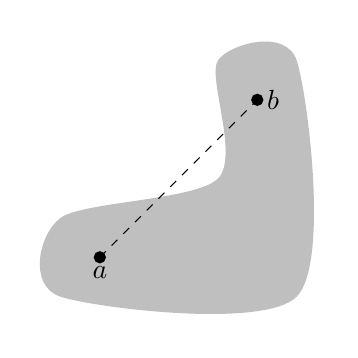
\begin{tikzpicture}

      \fill[lightgray] plot [smooth cycle] coordinates {
        (0, 0) (0, 1) (2, 1.5) (2, 3) (3, 3) (3, 0)
      };
      \draw[dashed] (0.5, 0.5) -- (2.5, 2.5);
      \draw[fill = black] (0.5, 0.5) circle (2pt) node[below] {\(a\)};
      \draw[fill = black] (2.5, 2.5) circle (2pt) node[right] {\(b\)};

    \end{tikzpicture}
  \caption{Невыпуклая область}\label{fig:area-prop-1-a}
  \end{subfigure}
  \qquad
  \begin{subfigure}[b]{0.2\textwidth}
    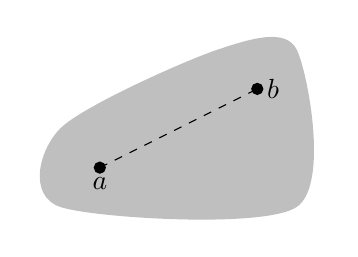
\begin{tikzpicture}

      \fill [lightgray] plot [smooth cycle] coordinates {
        (0, 0) (0, 1)  (2, 2) (3, 2) (3, 0)
      };
      \draw[dashed] (0.5, 0.5) -- (2.5, 1.5);
      \draw[fill = black] (0.5, 0.5) circle (2pt) node[below] {\(a\)};
      \draw[fill = black] (2.5, 1.5) circle (2pt) node[right] {\(b\)};

    \end{tikzpicture}
    \caption{Выпуклая область}\label{fig:area-prop-1-b}
  \end{subfigure}
\end{figure}
